\begin{frame}[fragile]{Unicycle Car Model}
\begin{columns}
    \column{0.35\textwidth}
    \begin{figure}
        \begin{center}
        \resizebox{0.9\columnwidth}{!}{
        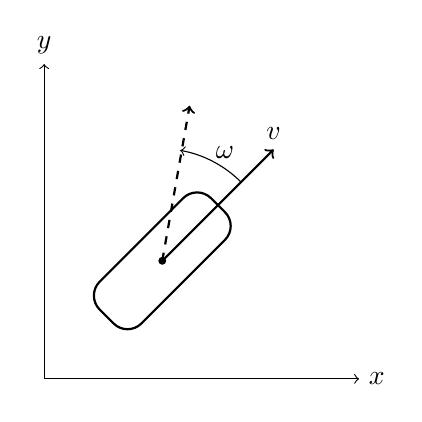
\begin{tikzpicture}
            % Define parameters
            \def\x{1.5}  % X-position of unicycle
            \def\y{1.5}  % Y-position of unicycle
            \def\width{0.75}  % Width of unicycle
            \def\height{2}  % Height of unicycle

            % Draw wheel
            \draw[thick, rounded corners=0.25cm, rotate around={-45:(\x,\y)}]({\x - 0.5*\width}, {\y - 0.5*\height}) rectangle ({\x + 0.5*\width}, {\y + 0.5*\height});

            \fill[black] (\x,\y) circle (0.05cm);

            % Draw the velocity vector from the center
            \draw[black, thick, ->] (\x,\y) -- ++(45:2) node[above] {$v$};
            \draw[black, thick, dashed, ->] (\x,\y) -- ++(80:2);

            % Draw an arc between the two vectors
            \draw[black, thin, ->] (\x+1,\y+1) arc (45:80:1.45) node[pos=0.3, above] {$\omega$};
            
            % Axes
            \draw[->] (0,0) -- (4,0) node[right] {$x$};
            \draw[->] (0,0) -- (0,4) node[above] {$y$};
        
        \end{tikzpicture}}
        \end{center}
    \end{figure}

    \column{0.65\textwidth}
    The state variables are $\vec{x} = (x, y, \omega, v)$. We define the neural feedback system $\mathcal{U}$ as follows:
    \[
        \langle 4, I^\mathcal{U}, F^\mathcal{U}, E^\mathcal{U}, u^\mathcal{U}, 0.2, 50, G^\mathcal{U}, \emptyset \rangle
    \]

    $I^\mathcal{U} = [9.5,9.55] \times [-4.5,-4.45] \times [2.1,2.11] \times [1.5,1.51]$, 
    \[
        F^\mathcal{U} = (\vec{x}_4 \cos(\vec{x}_3), \quad \vec{x}_4 \sin(\vec{x}_3), \quad 0, \quad 0)
    \]
    $E^\mathcal{U}=\{0\}\times\{0\}\times\{0\}\times [-10^{-4},10^{-4}]$, 
    $G^\mathcal{U} = [-0.6,0.6] \times [-0.2,0.2] \times [-0.06,0.06] \times [-0.3,0.3]$,
    $u^\mathcal{U}$ is a ReLU neural network with one hidden layer, $500$ neurons, and four outputs.

\end{columns}
\end{frame}